\begin{block}{case study: norfolk, va}
    We model a \emph{hypothetical} house in Norfolk, VA, where sea level rise drives nonstationary future flood hazard, following the approach of ref.~\cite{zarekarizi_suboptimal:2020}.
    \begin{framed}
        \begin{figure}
            \centering
            \includegraphics[width=\textwidth]{historic_surge.pdf}
            \caption{
                Time series of annual maximum storm surges (after subtracting mean sea level) at Sewells Point, VA.
                Purple (orange) arrows denote notable tropical cyclones (nor'easters).
            }
            \label{fig:observations}
        \end{figure}
    \end{framed}
    \vspace*{-1em}
    \begin{framed}
        \begin{figure}
            \centering
            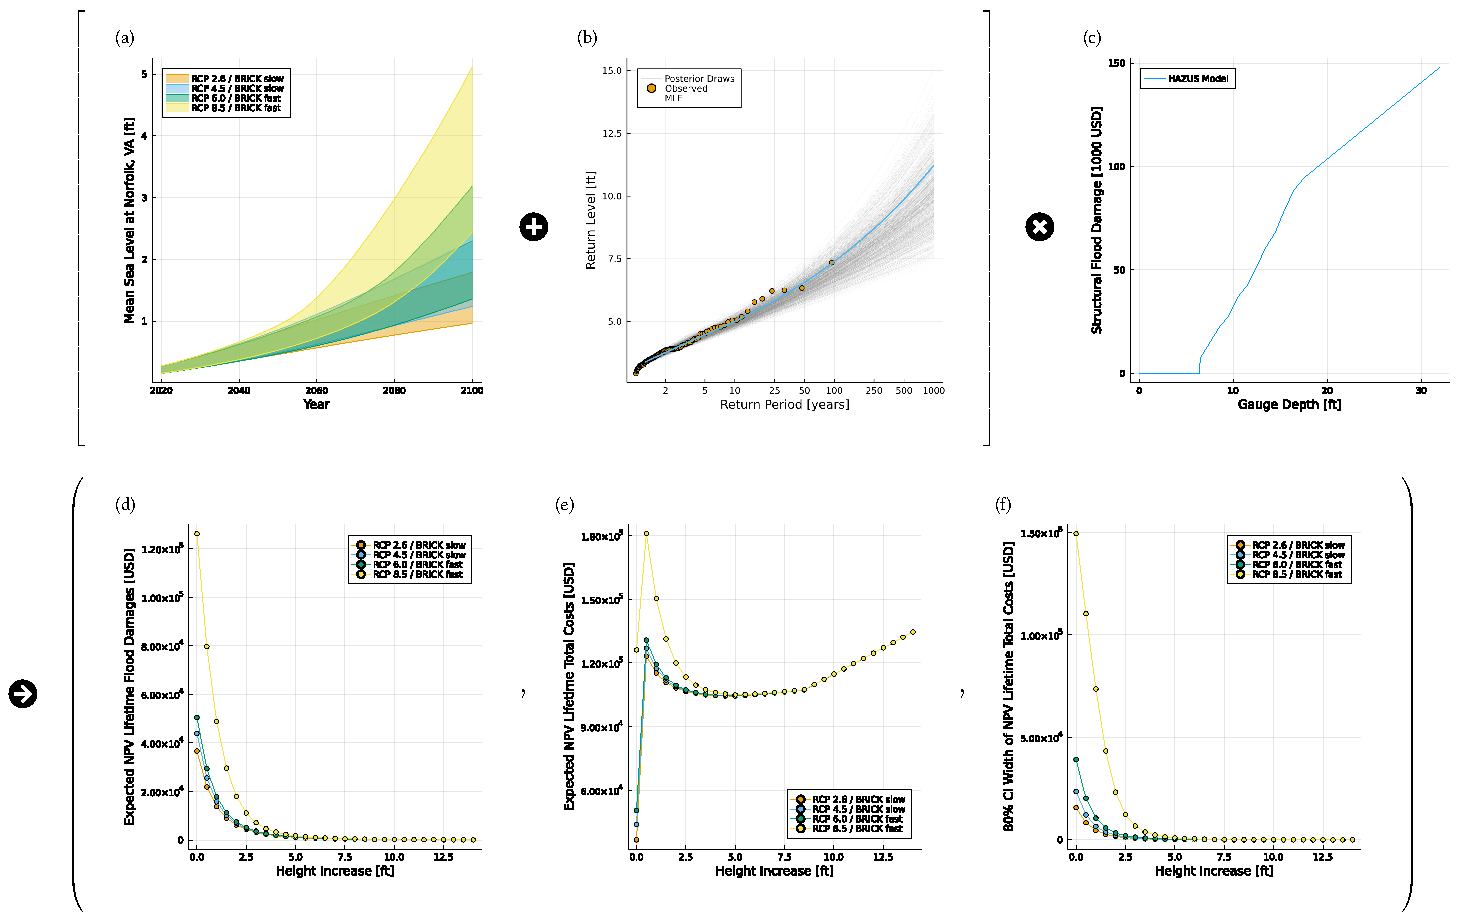
\includegraphics[width=\textwidth]{hazard-tradeoffs.pdf}
            \caption{
                Neglecting hydrodynamics, we add sea level rise (a) to a Bayesian GEV model of storm surge (b) to get flood hazard.
                The convolution of hazard and fragility (c) yields an assessment of damages and tradeoffs (\cref{fig:tradeoffs}).
            }
        \end{figure}
    \end{framed}
\end{block}